\documentclass[final]{siamltexmm}
\documentclass[10pt,a4paper]{article}

\usepackage{graphicx}
\usepackage{algorithm}
\usepackage{algorithmic}

% \usepackage[demo]{graphicx}
% \usepackage{subfig}

\newcommand{\pe}{\psi}
\def\d{\delta} 
\def\ds{\displaystyle} 
\def\e{{\epsilon}} 
\def\eb{\bar{\eta}}  
\def\enorm#1{\|#1\|_2} 
\def\Fp{F^\prime}  
\def\fishpack{{FISHPACK}} 
\def\fortran{{FORTRAN}} 
\def\gmres{{GMRES}} 
\def\gmresm{{\rm GMRES($m$)}} 
\def\Kc{{\cal K}} 
\def\norm#1{\|#1\|} 
\def\wb{{\bar w}} 
\def\zb{{\bar z}} 

% some definitions of bold math italics to make typing easier.
% They are used in the corollary.

\def\bfE{\mbox{\boldmath$E$}}
\def\bfG{\mbox{\boldmath$G$}}

\title{Deep Learning Assignment 1}
\author{Yun-shao Sung\thanks{\tt yss265@nyu.edu}
        \and Chung-Ling Yao\thanks{\tt cly264@nyu.edu}}

\begin{document}
\maketitle

\begin{abstract}
This is the report for deep learning assignment 1
\end{abstract}

\pagestyle{myheadings}
\thispagestyle{plain}

\section{Warmup}
Write $\partial E \over \partial X_{in} $ in terms of $\partial E \over \partial X_{out} $
\begin{equation}
{\partial E\over \partial X_{in}} = {\partial E\over \partial X_{out}} {\partial F(X_{in}, W_i) \over \partial X_{in}} = {\partial E\over \partial X_{out}} {e^{X_{in}} \over (1+e^{X_{in}})^2} = {\partial E\over \partial X_{out}} X_{out} (1-X_{out})
\end{equation}

\\
\section{Multinomial logistic regression}
Write the expression of ${\partial (X_{out})_i \over \partial (X_{in})_j}$ 
\\ if $i = j$, , and let $C = \displaystyle\sum_{k} e^{(X_I)_k}} - e^{(X_I)_i$
\begin{equation}
(X_o)_i = {{ e^{(X_I)_i}\over \displaystyle\sum_{k} e^{(X_I)_k}} = {{ e^{(X_I)_i}\over e^{(X_I)_0} + e^{(X_I)_i} + \ldots e^{(X_I)_i} + \ldots + e^{(X_I)_k}} = {{ e^{(X_I)_i}\over C + e^{(X_I)_i}}
\end{equation}
\begin{equation}
{\partial (X_o)_i\over \partial (X_I)_i} = {\partial \over \partial (X_I)_i} \Bigg({{ e^{(X_I)_i}\over C + e^{(X_I)_i}} \Bigg) = {{ -\beta e^{-\beta(X_I)_i}\over C + e^{(X_I)_i}} +  { \beta e^{-2\beta(X_I)_i}\over {(C + e^{(X_I)_i}})^2} } = \beta X_{o}(-1+X_{o})
\end{equation}
\\
\\if $i \neq j$, and let $K = \displaystyle\sum_{k} e^{(X_I)_k}} - e^{(X_I)_j$
\begin{equation}
{\partial (X_o)_i\over \partial (X_I)_j} = {\partial \over \partial (X_I)_j} \Bigg({{ e^{(X_I)_i}\over K + e^{(X_I)_j}} \Bigg) = {{ \beta e^{-\beta(X_I)_i} e^{-\beta(X_I)_j}\over {(K + e^{(X_I)_i}})^2} = \beta(X_o)_i (X_o)_j
\end{equation}


\\
\section{Torch (MNIST Handwritten Digit Recognition)}

\subsection{Experiment}

\subsubsection{Original Model}
The training and test accuracy of the original model. In the following experiments, we will compare the outcome of different configure with the original model. 
The training accuracy achieve 100\% in epoch 30. The test accuracy shift up and down slightly, but it increase in long term. 

\begin{table}[H]
\begin{center}
    \begin{tabular}{| c | c | c |}
    \hline
    Epoch & Training Accuracy (\%) & Test Accuracy (\%) \\ \hline
    1 & 96.71 & 99.04 \\ \hline
    2 & 99.04 & 99.41 \\ \hline
    3 & 99.34 & 99.40 \\ \hline
    4 & 99.53 & 99.47 \\ \hline
    5 & 99.62 & 99.48 \\ \hline
    6 & 99.77 & 99.54 \\ \hline
    7 & 99.81 & 99.48 \\ \hline
    8 & 99.86 & 99.43 \\ \hline  
    9 & 99.89 & 99.49 \\ \hline
    10 & 99.92 & 99.51 \\ \hline      
    \end{tabular}
\end{center}
\caption{The training and test accuracy of the original model}
\end{table}


\subsubsection{Different normalization methods}
Use different normalization methods, such as different Gaussian 1D normalization array size or without normalization. Virtualize it to see the effect on the images, and compare the training/test accuracy in the first three epoches.

\begin{table}[H]
\newcommand{\tabincell}[2]{\begin{tabular}{@{}#1@{}}#2\end{tabular}}
\begin{center}
    \begin{tabular}{| c | c | c | c | c | c | c |}
    \hline
    Normalization 
    	& \multicolumn{2}{|c|}{Gaussian1D(7)} 
    	& \multicolumn{2}{|c|}{Gaussian1D(15)} & \multicolumn{2}{|c|}{no normalization} \\ \hline
    \tabincell{c}{Vitualization}
    	& \multicolumn{2}{|c|}{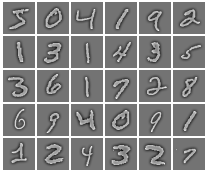
\includegraphics[width=3cm,height=3cm,trim=0 0 0 -1]{../fig/g7.png}} 
    	& \multicolumn{2}{|c|}{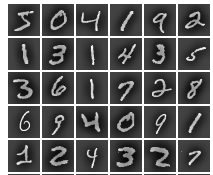
\includegraphics[width=3cm,height=3cm,trim=0 0 0 -1]{../fig/g15.png}} 
    	& \multicolumn{2}{|c|}{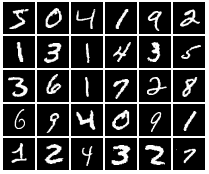
\includegraphics[width=3cm,height=3cm,trim=0 0 0 -1]{../fig/no.png}} \\ \hline
    \tabincell{c}{Accuracy in \\ each epoch} & training & test & training & test & training & test \\ \hline
    1 & 96.71 & 99.04 & 96.72 & 98.88 & 96.66 & 98.79 \\ \hline
    2 & 99.04 & 99.41 & 99.00 & 99.11 & 98.99 & 99.14 \\ \hline
    3 & 99.34 & 99.40 & 99.32 & 99.28 & 99.27 & 99.31 \\ \hline
    \end{tabular}
\end{center}
\caption{The training and test accuracy of different normalization methods}
\end{table}


\subsubsection{Different curve function}
The original curve function is tanh. We changed it to be reLU. We found the original tanh function works better in both training and test accuracy.

\begin{table}[H]
\newcommand{\tabincell}[2]{\begin{tabular}{@{}#1@{}}#2\end{tabular}}
\begin{center}
    \begin{tabular}{| c | c | c | c | c | c | c |}
    \hline
    Loss Function 
    	& \multicolumn{2}{|c|}{Tanh(default)} 
    	& \multicolumn{2}{|c|}{reLU} & \multicolumn{2}{|c|}{---} \\ \hline
    \tabincell{c}{Accuracy in \\ each epoch} & training & test & training & test & training & test \\ \hline
    1 & 96.71 & 99.04 & 96.52 & 98.73 & XX.XX & XX.XX \\ \hline
    2 & 99.04 & 99.41 & 98.86 & 99.02 & XX.XX & XX.XX \\ \hline
    3 & 99.34 & 99.40 & 99.13 & 99.08 & XX.XX & XX.XX \\ \hline
    \end{tabular}
\end{center}
\caption{The training and test accuracy of different curve function}
\end{table}


\subsubsection{Different loss function}
The original loss function is NLL. We changed it to multi-margin and MSE. We find the multi-margin 
generate the same result with NLL. The MSE looks slightly better in training accuracy, but not in test accuracy.

\begin{table}[H]
\newcommand{\tabincell}[2]{\begin{tabular}{@{}#1@{}}#2\end{tabular}}
\begin{center}
    \begin{tabular}{| c | c | c | c | c | c | c |}
    \hline
    Loss Function 
    	& \multicolumn{2}{|c|}{NLL(default)} 
    	& \multicolumn{2}{|c|}{Multi-margin} & \multicolumn{2}{|c|}{MSE} \\ \hline
    \tabincell{c}{Accuracy in \\ each epoch} & training & test & training & test & training & test \\ \hline
    1 & 96.71 & 99.04 & 96.71 & 99.04 & 96.74 & 99.04 \\ \hline
    2 & 99.04 & 99.41 & 99.04 & 99.41 & 99.07 & 99.30 \\ \hline
    3 & 99.34 & 99.40 & 99.34 & 99.40 & 99.35 & -- \\ \hline
    \end{tabular}
\end{center}
\caption{The training and test accuracy of different loss function}
\end{table}


\subsubsection{Different model structure}


\end{document}
